%\documentclass[a4paper,12pt,twoside]{book}
\documentclass[12pt,times]{report}
\usepackage{mathptmx}%This package supersedes times and mathptm
\usepackage[a4paper,right=2.54cm,left=2.54cm,top=2.54cm,bottom=2.54cm]{geometry}

%%%%paquete para usar citas de diferentes formatos
%%%%%%%%%%%%%%%%%%%%%%%%%%%%%%%%%
%%add al indice
%\usepackage[nottoc,numbib]{tocbibind}
%\usepackage[authoryear,round]{natbib}
\usepackage[utf8]{inputenc}
\usepackage{csquotes}
\usepackage[spanish]{babel}
\usepackage[style=apa ,
%hyperref=auto,
%citestyle=authoryear,
natbib=true,
backend=biber]{biblatex}
\addbibresource{biblio/references.bib}
%\usepackage{biblatex}
%paquete para hiperlinks entre citas e imagenes
%%%%%%%%%%%%%%%%%%%%%%%%%%%%%%%%%
\usepackage[colorlinks=true,
citecolor=blue,
urlcolor=cyan,
bookmarks=true,
linkcolor=blue,
pdftitle={Tesis-nombre-alumno},
pdfauthor={autor nombres}]{hyperref}

\usepackage{amssymb}
\usepackage{graphicx} % for improved inclusion of graphics
%\usepackage{wrapfig} % to include figure with text wrapping around it
\usepackage[margin=10pt,font=small,labelfont=bf]{caption} % for improved layout of figure captions with extra margin, smaller font than text
\usepackage{eucal}
\usepackage[usenames, dvipsnames]{color}
\usepackage[perpage]{footmisc}
%\usepackage[round, sort]{natbib}
\usepackage{ifthen}
\usepackage{multicol} % for pages with multiple text columns, e.g. References
\setlength{\columnsep}{20pt} % space between columns; default 10pt quite narrow
\usepackage[nottoc]{tocbibind} % correct page numbers for bib in TOC, nottoc suppresses an entry for TOC itself
\usepackage{appendix}

%%%----Modificar encabezado y pie de pagina
%%%%%%%%%%%%%%%%%%%%%%%%%%%%%%%%%%%%%%%%%%%%%%%%%%%%%%%%%%%%%%%%%%%%%
\usepackage{fancyhdr} % for better header layout
\newcommand{\changefont}{%
	\fontsize{9pt}{1.5pt}\selectfont
}
\pagestyle{fancy}
\fancyhf{} %% delete default configuration of page
%%\setlength\headheight{15pt}
\fancyhead[L]{\changefont Titulo de tesis aqui}
\fancyhead[R]{\changefont \leftmark}
%%\fancyfoot[L]{\leftmark}
\fancyfoot[R]{\thepage}

%%%%%%%%%%%%%%%%%%%%%%%%%%%%%5
%%%% Configuracion de los parrafos
%\usepackage{setspace}
%\onehalfspacing
%\linespread{1.25} 
\setlength{\parindent}{0.5in} %%sangria
\setlength{\parskip}{3mm}  %%espacio entre parrafos
\linespread{1.3} %This equals 1.5 linespacing in Word
%%%% nuevo parrafo
%%%%%%%%%%%%%%%%%%%%%%%%%%%%%5
%%%% Centrar valores de una tabla
\usepackage{array}
%%CENTRADO HORIZONTAL
\newcolumntype{P}[1]{>{\centering\arraybackslash}p{#1}}
%%CENTRADO VERTICAL
\newcolumntype{M}[1]{>{\centering\arraybackslash}m{#1}}

%%%%%%%%%%%%%%%%%%%%%%%%%%%%%5
%%%%Paquete para alinear texto
\usepackage{ragged2e}
\usepackage{multirow}
\usepackage{makecell}
\usepackage{rotating}
\usepackage{siunitx} % To align the numbers later on
\usepackage[table,xcdraw]{xcolor}
\usepackage{color, colortbl}
\definecolor{Gray}{gray}{0.9}
\definecolor{orange}{rgb}{1,0.647,0}
\definecolor{turq3}{rgb}{0.54, 0.81, 0.94}
\definecolor{turq}{rgb}{0.63, 0.79, 0.95}
\definecolor{bluejean}{rgb}{0.03, 0.27, 0.49}

%%%%%%%%%%%%%%%%%%%%%%%%%
\usepackage{xparse}
\usepackage{expl3}
%%%%funcion de reemplazar regex
\ExplSyntaxOn
\NewDocumentCommand{\replace}{mmm}
{
	\marian_replace:nnn {#1} {#2} {#3}
}

\tl_new:N \l_marian_input_text_tl
\tl_new:N \l_marian_search_tl
\tl_new:N \l_marian_replace_tl

\cs_new_protected:Npn \marian_replace:nnn #1 #2 #3
{
	\tl_set:Nn \l_marian_input_text_tl { #1 }
	\tl_set:Nn \l_marian_search_tl { #2 }
	\tl_set:Nn \l_marian_replace_tl { #3 }
	\regex_replace_all:nnN { \b\u{l_marian_search_tl}\b } { \u{l_marian_replace_tl} } \l_marian_input_text_tl
	\tl_use:N \l_marian_input_text_tl
}
\ExplSyntaxOff

%%%%%%%%%%%%%%%%%%%%%%%%%%%%%%%%%%%%%%
\usepackage{amsmath}
\numberwithin{equation}{chapter} %%enumerar ecuaciones
\renewcommand{\theequation}{Ecuación \thechapter.\arabic{equation}}   
\usepackage{mathtools, nccmath, cool}
%%%Configuraciones de biblatex

%\include{biblio/config}
\makeatletter
\let\abx@macro@citeOrig\abx@macro@cite
\renewbibmacro{cite}{%
	\bibhyperref{%
		\let\bibhyperref\relax\relax%
		\abx@macro@citeOrig%
	}%
}
\let\abx@macro@textciteOrig\abx@macro@textcite
\renewbibmacro{textcite}{%
	\bibhyperref{%
		\let\bibhyperref\relax\relax%
		\abx@macro@textciteOrig%
	}%
}%

\makeatother

%%%%%%%%%%%%%%%%%%%%%%%%%%%%%%%%%%%%%%%%%%%
\begin{document}

\begin{titlepage}

	\begin{center}
		%%%cargar imagen
	    \includegraphics[width=0.45\textwidth]{images_repo/esanlogomin}
		\vspace*{2cm} \\
		UNIVERSIDAD ESAN \vspace*{1ex} \\
		FACULTAD DE INGENIERÍA \vspace*{1ex} \\
		INGENIERÍA DE TECNOLOGÍAS DE INFORMACIÓN Y SISTEMAS\vspace*{8ex} \\
		\textbf{Evaluación de Modelos de Deep Learning para la Detección Temprana de Retinopatía Diabética}
		\vspace*{8ex}\\	
		Trabajo de investigación para el curso de Trabajo de Tesis I 
		\vspace*{8ex} \\	
		Arroyo Almonacid José Eduardo \\
		Asesor: Marks Calderón		
		\vfill
		
		Lima, \today 
		
	\end{center}
\end{titlepage}
%%cambiar nombres de objetos para el indice y otros
\renewcommand{\listfigurename}{Índice de Figuras}
\renewcommand{\tablename}{Tabla}
\renewcommand{\listtablename}{Índice de Tablas}

\include{0/resumen}
\include{0/abstract}
\include{0/dedicacion}
\include{0/agradecimientos}

% outline
\tableofcontents            % print the table of contents

%: ----------------------- contents ------------------------

\setcounter{secnumdepth}{3} % organisational level that receives a numbers
\setcounter{tocdepth}{3}    % print table of contents for level 3

% levels are: 0 - chapter, 1 - section, 2 - subsection, 3 - subsection


%: ----------------------- list of figures/tables ------------------------

\listoffigures	% print list of figures

\listoftables  % print list of tables



\chapter{PLANTEAMIENTO DEL PROBLEMA}
\section{Descripción de la Realidad Problemática}

La retinopatía diabética (RD) constituye una complicación severa derivada de la diabetes, siendo la principal causa de pérdida de visión en adultos trabajadores en naciones desarrolladas. Esta afección impacta profundamente en la vida de las personas, no solo reduciendo su calidad de vida por la disminución visual, sino también imponiendo retos económicos significativos para los sistemas de salud debido al elevado precio de los tratamientos.

Globalmente, más de 537 millones de adultos viven con diabetes, y se estima que este número ascenderá a más de 780 millones para el año 2045. Un análisis exhaustivo muestra que alrededor del 34.6\% de estas personas desarrollarán alguna forma de RD, y un 7\% experimentará variantes severas como la retinopatía diabética proliferativa.

\begin{figure}[h]
    \centering
    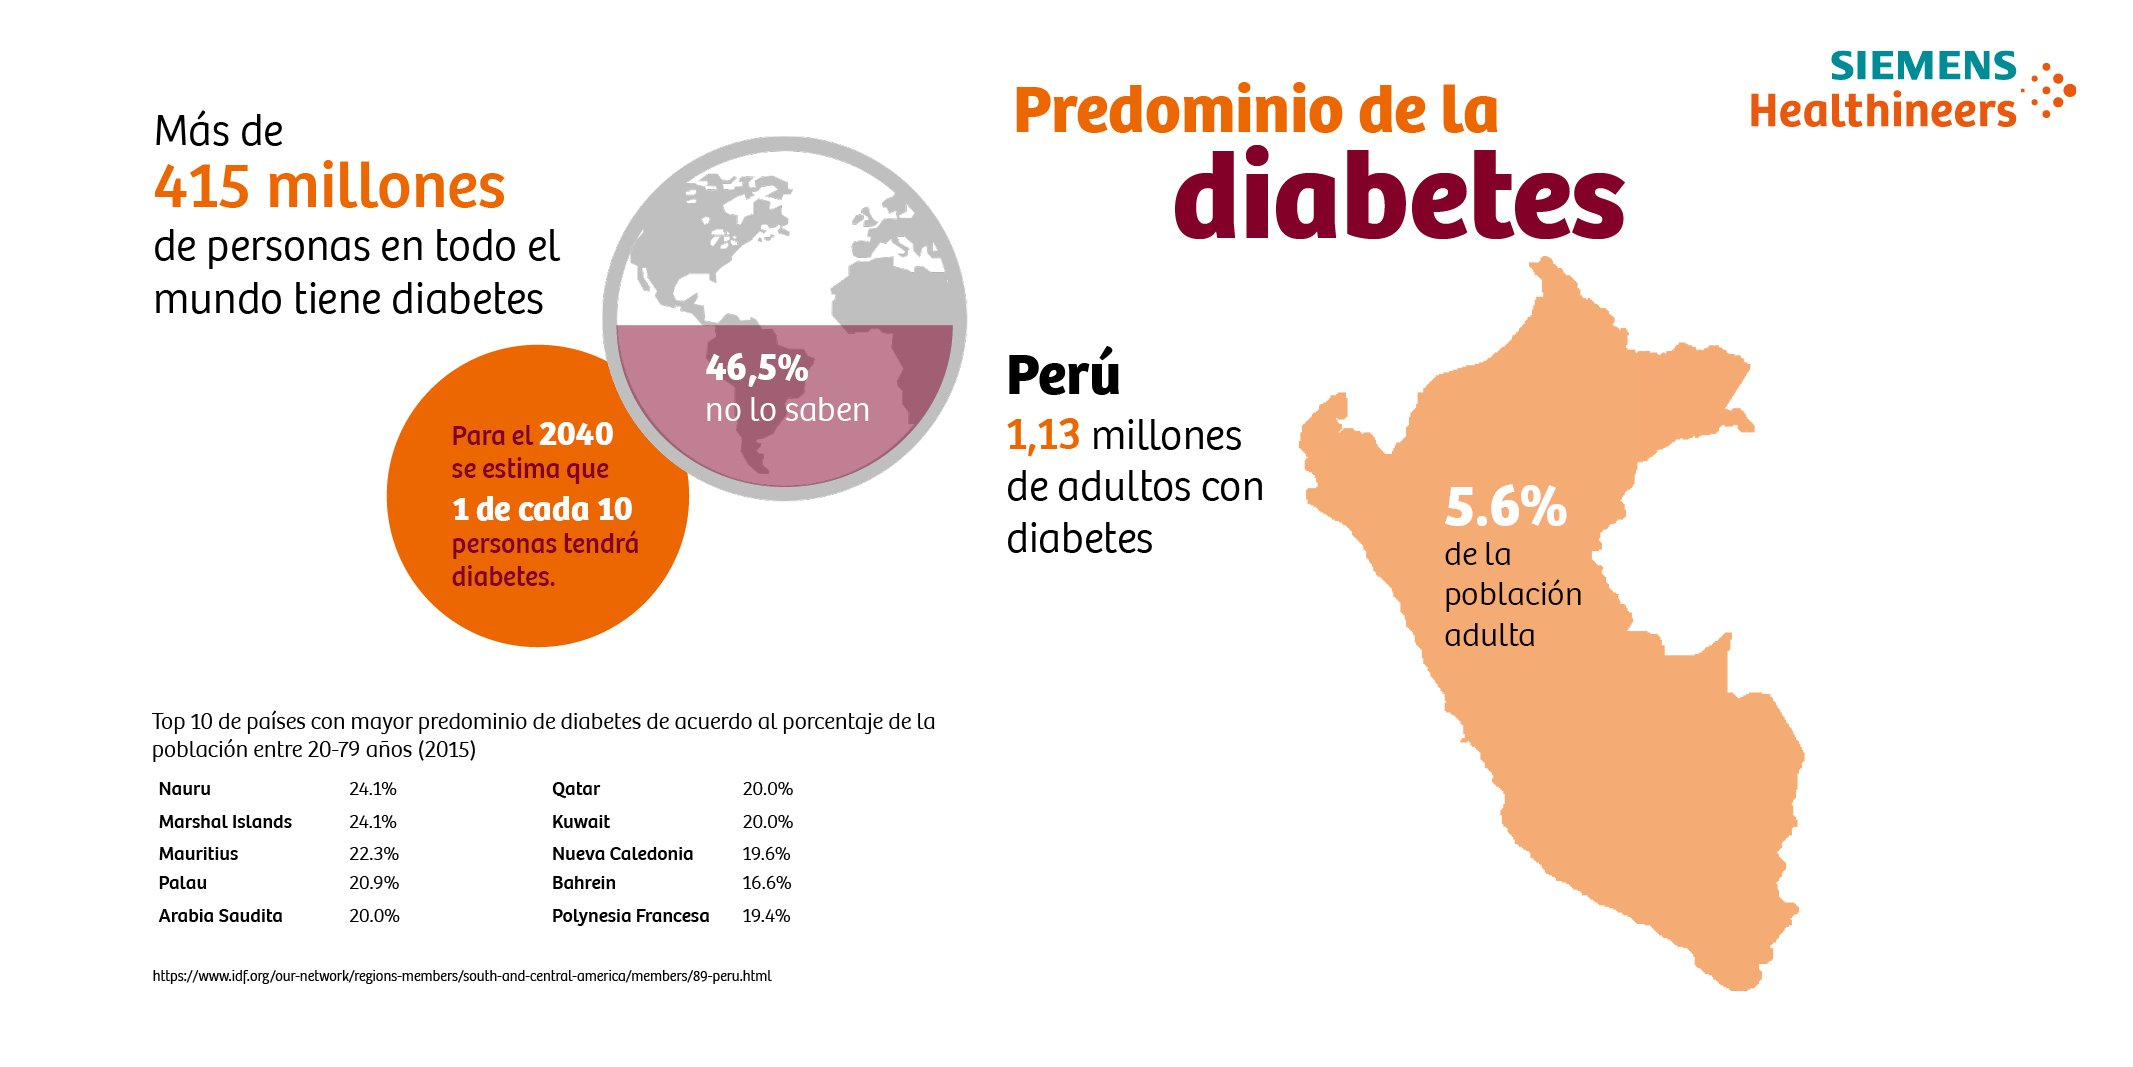
\includegraphics[width=0.8\textwidth]{images_repo/Predominiodeladiabetes.jpg}
    \caption{Predominio de la diabetes en Perú. Fuente: \cite{idf2021}}
    \label{fig:diabetes_peru}
\end{figure}

La repercusión socioeconómica de la RD es vasta, incluyendo no solo los costes directos de los tratamientos sino también la reducción de la capacidad laboral de los afectados, lo que puede llevar a la pérdida de autonomía y al desarrollo de trastornos emocionales. Las opciones de tratamiento avanzadas, como las inyecciones intraoculares y las intervenciones quirúrgicas retinianas, suponen un lastre económico adicional tanto para los pacientes como para los sistemas sanitarios.

\textbf{Acceso Desigual a la Atención Médica}

Existen notables disparidades en el acceso a los servicios médicos que pueden influir significativamente en la detección y tratamiento oportunos de la RD. Estas variaciones son particularmente evidentes entre distintas regiones y estratos socioeconómicos, y requieren ser abordadas en las políticas de salud para garantizar un tratamiento equitativo.

\textbf{Impacto Psicológico y Comunitario}

El deterioro visual grave resultante de la RD afecta no solo a nivel individual, sino que también repercute en el entorno familiar y comunitario del paciente, exacerbando problemas psicosociales como el estrés y la depresión.

\textbf{Costos Económicos a Nivel Macro y Micro}

Además de los gastos médicos directos, la RD acarrea costos indirectos por la pérdida de productividad laboral. Analizar estos aspectos desde una perspectiva global y local ofrece un panorama más claro para diseñar intervenciones efectivas y contextualizadas.

\textbf{Innovaciones Tecnológicas en Detección y Tratamiento}

La revolución tecnológica en la salud ha introducido herramientas como la inteligencia artificial y la telemedicina, las cuales están cambiando la forma de diagnóstico y tratamiento de la RD. Estas innovaciones presentan nuevas oportunidades pero también desafíos, particularmente en términos de acceso equitativo.

\textbf{Políticas Públicas y Estrategias de Prevención}
Es esencial evaluar críticamente las políticas y estrategias de salud pública vigentes, identificando áreas de mejora para fortalecer la prevención y el tratamiento de la RD, a través de campañas más efectivas y programas de detección mejorados.

\textbf{Futuro y Sostenibilidad del Sistema de Salud}

Ante el incremento esperado en la prevalencia de la diabetes, es imperativo que los sistemas de salud se preparen para manejar esta carga creciente de manera eficiente y sostenible.

\section{Problema General}
\newcommand{\ProblemaGeneral}{
	¿De qué manera la implementación de un modelo de deep learning adecuado puede mejorar los resultados de los pre-diagnósticos de retinopatía diabética?
}
\ProblemaGeneral

\subsection{Problemas Específicos}
\newcommand{\Pbone}{
	¿Qué datos serán necesarios para entrenar modelos de deep learning en la pre-detección de la retinopatía diabética?
}
\newcommand{\Pbtwo}{
	¿Cuál será la arquitectura de modelo de deep learning más efectiva para identificar características tempranas de la retinopatía diabética?
}
\newcommand{\Pbthree}{
	¿Qué métodos de preprocesamiento de imágenes serán utilizados para mejorar la precisión del modelo de deep learning en la detección de retinopatía diabética?

}
\newcommand{\Pbfour}{
	¿Qué métricas serán utilizadas para evaluar y comparar la efectividad de diferentes modelos de deep learning en la detección de la retinopatía diabética?
}
\newcommand{\Pbfive}{
	ES
}

\begin{itemize}
	\item \Pbone
	\item \Pbtwo
	\item \Pbthree
	 \item \Pbfour
	% \item \Pbfive
\end{itemize}

\section{Objetivos de la Investigación}

\subsection{Objetivo General}
\newcommand{\ObjetivoGeneral}{
	Evaluar la implementación de un modelo de deep learning para mejorar los resultados de los pre-diagnósticos de retinopatía diabética.
}
\ObjetivoGeneral

\subsection{Objetivos Específicos}
\newcommand{\Objone}{
	Identificar los datos necesarios para entrenar modelos de deep learning en la pre-detección de la retinopatía diabética.
}
\newcommand{\Objtwo}{
	Determinar la arquitectura de modelo de deep learning más efectiva para identificar características tempranas de la retinopatía diabética.
}
\newcommand{\Objthree}{
	Evaluar los métodos de preprocesamiento de imágenes que mejoren la precisión del modelo de deep learning en la detección de retinopatía diabética.
}
\newcommand{\Objfour}{
	Definir y utilizar métricas para evaluar y comparar la efectividad de diferentes modelos de deep learning en la detección de la retinopatía diabética.
}
\newcommand{\Objfive}{

}

\begin{itemize}
	\item \Objone
	\item \Objtwo
	\item \Objthree
	 \item \Objfour
	% \item \Objfive
\end{itemize}

\section{Justificación de la Investigación}

\subsection{Teórica}

Este estudio se centra en la implementación de modelos de aprendizaje profundo para la detección temprana de la retinopatía diabética, una complicación prevalente y grave entre los diabéticos en Perú. Investigaciones recientes indican que la prevalencia de la retinopatía diabética en pacientes con diabetes tipo 2 es de 57.62\%, con una prevalencia de retinopatía diabética no proliferativa de 47.29\% y retinopatía diabética proliferativa de 10.33\% \cite{yanhez2016prevalencia}. Este proyecto busca profundizar el entendimiento de cómo los avances en inteligencia artificial pueden mejorar significativamente la detección y el seguimiento precoz de esta afección. 

La aplicación de técnicas avanzadas de aprendizaje profundo tiene el potencial de revolucionar la manera en que se detectan y manejan las enfermedades oculares. En el caso de la retinopatía diabética, los modelos de deep learning pueden ofrecer una precisión y eficiencia superiores en la identificación de signos tempranos, lo cual es crucial para la implementación de intervenciones oportunas. Este estudio no solo pretende validar la efectividad de estos modelos en un entorno clínico, sino también explorar sus limitaciones y desafíos asociados con su implementación \cite{huang2023advances}.


\subsection{Práctica}
Desde un punto de vista práctico, este trabajo de investigación tiene el potencial de generar una mejora considerable en el método de pre-detección de la retinopatía diabética en Perú, donde comúnmente el diagnóstico ocurre en fases muy avanzadas. Implementar modelos de deep learning para la identificación temprana de la enfermedad podría facilitar intervenciones preventivas más efectivas, aliviar la carga económica sobre el sistema de salud y mejorar significativamente los resultados para los pacientes. Integrar esta tecnología en los sistemas públicos de salud mejoraría la accesibilidad y eficacia del diagnóstico de la retinopatía diabética, especialmente en zonas donde los recursos son escasos. Estudios recientes sobre el uso de deep learning en la detección de enfermedades cardíacas han demostrado su eficacia y precisión, lo que sugiere que métodos similares podrían ser beneficiosos para la detección de la retinopatía diabética \cite{rajeswari2022heart, arulkumar2023monitoring}.


\subsection{Metodológica}
Metodológicamente, este estudio se distingue por su análisis exhaustivo y comparativo de diversos modelos de deep learning en función de su rendimiento con las variables comunes en el aprendizaje profundo y modelos predictivos. La metodología rigurosa que se aplicará no solo evaluará la precisión de estos modelos, sino que también explorará adaptaciones necesarias para maximizar su eficacia en el contexto específico de Perú.

Según \citet{sharma2020deep}, los modelos de deep learning han demostrado ser altamente efectivos en la detección de enfermedades utilizando imágenes médicas. Este enfoque se aplicará para evaluar cómo estos modelos pueden ser adaptados para la detección temprana de la retinopatía diabética.

Además, \citet{jiang2020heart} subrayan la importancia de ajustar los modelos de deep learning a los datos locales para mejorar su precisión y rendimiento. Esta investigación se centrará en adaptar y optimizar los modelos existentes para el contexto específico de Perú, proporcionando una base sólida para futuras aplicaciones en otras condiciones médicas y en el desarrollo de políticas de salud pública relacionadas con la implementación de nuevas tecnologías.




\section{Delimitación del Estudio}

\subsection{Espacial}
Este estudio se delimita al análisis de datos obtenidos de bases de datos internacionales reconocidas, específicamente el Messidor dataset y el APTOS 2019. Estas bases contienen imágenes de fondo de ojo de pacientes diabéticos, recolectadas bajo diversos estudios clínicos. La selección de estas bases de datos se debe a su amplio uso en la investigación académica y su relevancia para validar la precisión de modelos de deep learning en el contexto de la retinopatía diabética. Los tres modelos evaluados en este estudio incluyen el Customized Convolutional Neural Network (CCNN) de Mane et al. \cite{mane2023customized}, el modelo propuesto por Mohanty et al. \cite{mohanty2023using}, y el modelo de Deep Learning desarrollado por otro grupo de investigadores destacados en el campo \cite{huang2023advances}. La investigación no involucrará la recolección de nuevos datos clínicos ni se realizarán pruebas directas con pacientes en Perú o cualquier otra región, concentrándose exclusivamente en el análisis técnico y comparativo de los datos ya existentes.


\subsection{Temporal}
La investigación se llevará a cabo durante el año académico 2024, comenzando en enero y concluyendo en diciembre del mismo año. Este marco temporal ha sido seleccionado para alinear el estudio con el calendario académico, proporcionando un tiempo adecuado para cada fase del proyecto. Durante este período, se realizará la planificación detallada, la selección de modelos de deep learning, el procesamiento de datos, la ejecución de pruebas computacionales, y el análisis de los resultados. Este cronograma garantizará que todas las etapas del estudio se completen de manera organizada y eficiente.



\subsection{Conceptual}
La investigación está enfocada en la evaluación técnica de modelos de deep learning específicos que han sido previamente desarrollados y aplicados en la detección de la retinopatía diabética. La delimitación conceptual incluye la validación de la efectividad de estos modelos en términos de precisión, sensibilidad, especificidad y otras métricas relevantes para el diagnóstico automatizado mediante imágenes. Se excluyen del estudio la creación de nuevos modelos de inteligencia artificial, cualquier intervención médica directa con pacientes, y la exploración de tratamientos para la retinopatía diabética. Este enfoque permite una concentración rigurosa en la evaluación del rendimiento de tecnologías específicas en un contexto controlado y basado en datos, proporcionando una evaluación crítica de su utilidad práctica y sus limitaciones.


\section{Hipótesis}

\subsection{Hipótesis General}
\newcommand{\HipotesisGeneral}{
	La implementación de un modelo de deep learning adecuado mejorará significativamente los resultados de los pre-diagnósticos de retinopatía diabética.
}
\HipotesisGeneral

\subsection{Hipótesis Específicas}
\newcommand{\Hone}{
	Los datos seleccionados para entrenar modelos de deep learning serán suficientes y relevantes para mejorar la precisión en la pre-detección de la retinopatía diabética.
}
\newcommand{\Htwo}{
	La arquitectura de modelo de deep learning más efectiva identificará características tempranas de la retinopatía diabética con mayor precisión que las arquitecturas tradicionales.
}
\newcommand{\Hthree}{
	Los métodos de preprocesamiento de imágenes aplicados mejorarán la precisión del modelo de deep learning en la detección de la retinopatía diabética.
}
\newcommand{\Hfour}{
	Las métricas definidas y utilizadas para evaluar los modelos de deep learning proporcionarán una comparación clara y efectiva de la precisión y efectividad de diferentes modelos en la detección de la retinopatía diabética.
}
\newcommand{\Hfive}{
	xws
}

\begin{itemize}
	\item \Hone
	\item \Htwo
	\item \Hthree
	 \item \Hfour
	% \item \Hfive
\end{itemize}

\subsection{Matriz de Consistencia}
A continuación se presenta la matriz de consistencia elaborada para la presente investigación (véase Anexo \ref{1:table}).

\include{2/marco}
\include{3/metodologia}
\include{4/desarrollo}
\include{5/resultados}
\include{6/conclusion}
%%Anexos
\appendix
\renewcommand{\appendixname}{Anexos}
\renewcommand{\appendixtocname}{Anexos}
\renewcommand{\appendixpagename}{Anexos}
\clearpage
\addappheadtotoc
\appendixpage
\chapter{Anexo I: Matriz de Consistencia}

% Incluye la imagen de la primera parte de la matriz
\begin{figure}[h!]
	\centering
	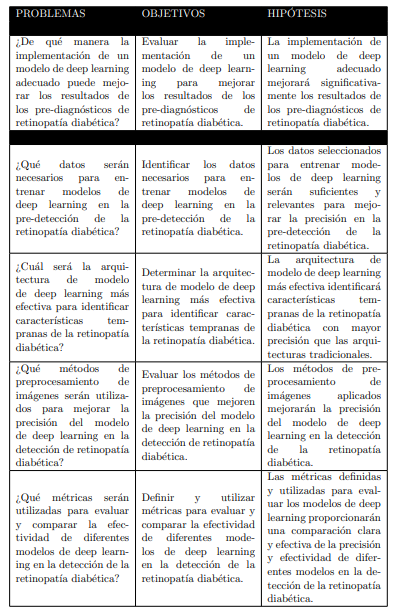
\includegraphics[width=\textwidth]{C:/Users/José Arroyo/Desktop/tesis cambios/TesisJoseArroyo/images_repo/MATRIZ PARTE 1.png}
	\caption{Matriz de consistencia (Parte 1). Fuente: Elaboración propia}
	\label{fig:matriz_parte1}
\end{figure}

% Incluye la imagen de la segunda parte de la matriz
\begin{figure}[h!]
	\centering
	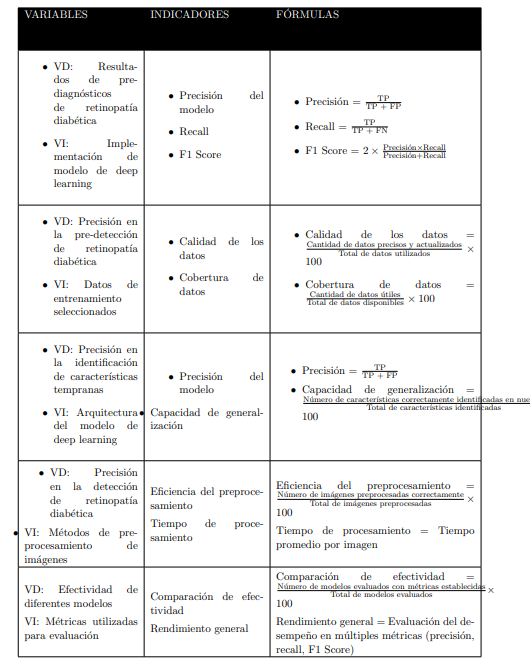
\includegraphics[width=\textwidth]{C:/Users/José Arroyo/Desktop/tesis cambios/TesisJoseArroyo/images_repo/MATRIZ PARTE 2.png}
	\caption{Matriz de consistencia (Parte 2). Fuente: Elaboración propia}
	\label{fig:matriz_parte2}
\end{figure}

\chapter{Anexo II: Árbol de Problemas}

% Incluye la imagen del árbol de problemas
\begin{figure}[h!]
	\centering
	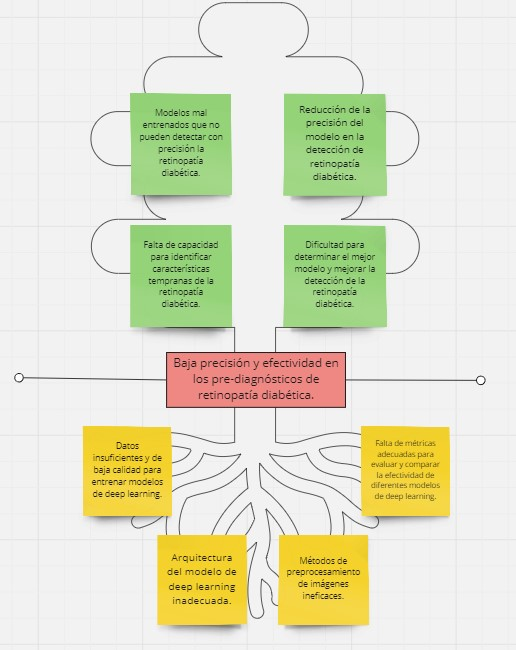
\includegraphics[width=\textwidth]{C:/Users/José Arroyo/Desktop/tesis cambios/TesisJoseArroyo/images_repo/Arbol de problemas miro.jpg}
	\caption{Árbol de Problemas. Fuente: Elaboración propia}
	\label{fig:arbol_problemas}
\end{figure}

\chapter{Anexo III: Resumen de Papers Investigados}

\begin{table}[h!]
	\centering
	\footnotesize
	\begin{tabular}{|p{0.5cm}|p{0.3cm}|p{4cm}|p{2cm}|p{0.6cm}|p{1.7cm}|p{3cm}|}
		\hline
		\rowcolor{bluejean} \multicolumn{1}{|c|}{\textcolor{white}{Tipo}} & \multicolumn{1}{c|}{\textcolor{white}{N°}} & \multicolumn{1}{c|}{\textcolor{white}{Título}} & \multicolumn{1}{c|}{\textcolor{white}{Autor}} & \multicolumn{1}{c|}{\textcolor{white}{Año}} & \multicolumn{1}{c|}{\textcolor{white}{País}} & \multicolumn{1}{c|}{\textcolor{white}{Fuente}} \\
		\hline
		\multirow{2}{*}{\rotatebox[origin=c]{90}{Problema}} & 1 & Deep Convolutional Neural Networks for Detecting COVID-19 Using Medical Images: A Survey & Sharma, et al. & 2020 & India & \textit{IEEE Access} \\
		\cline{2-7}
		& 2 & Heart Disease Detection Using Machine Learning and Deep Learning Techniques & Jiang, et al. & 2020 & USA & \textit{International Journal of Medical Informatics} \\
		\hline
		\multirow{3}{*}{\rotatebox[origin=c]{90}{Propuesta}} & 3 & Monitoring and Recognition of Heart Health using Heartbeat Classification with Deep Learning and IoT & Arulkumar, et al. & 2023 & India & \textit{Journal of Machine and Computing} \\
		\cline{2-7}
		& 4 & Advances in Deep Learning: From Diagnosis to Treatment & Huang, et al. & 2023 & China & \textit{BioScience Trends} \\
		\cline{2-7}
		& 5 & A Study on Scope of Artificial Intelligence in Diagnostic Medicine & Santhosh Kumar, et al. & 2023 & India & \textit{IEEE Access} \\
		\hline
		\multirow{3}{*}{\rotatebox[origin=c]{90}{Otros}} & 6 & A Diabetic Retinopathy Detection using Customized Convolutional Neural Network & Mane, et al. & 2023 & India & \textit{International Journal of Electrical and Electronics Research} \\
		\cline{2-7}
		& 7 & Using Deep Learning Architectures for Detection and Classification of Diabetic Retinopathy & Mohanty, et al. & 2023 & India & \textit{Sensors} \\
		\cline{2-7}
		& 8 & Prevalencia de la retinopatía diabética y factores de riesgo asociados & Yáñez, et al. & 2016 & Peru & \textit{Revista Médica Carrionica} \\
		\hline
	\end{tabular}
	\caption{Cuadro Resumen de Papers Investigados. Fuente: Elaboración propia}
	\label{A:table}
\end{table}

\end{document}

% %%Bibliografia
%\bibliographystyle{apalike} % Title is link if provided
%\renewcommand{\bibname}{BIBLIOGRAFÍA} % changes the header; default: Bibliography

\printbibliography[heading=bibintoc,title={BIBLIOGRAFÍA}]
%\bibliography{biblio/references} % adjust this to fit your BibTex file
\end{document}